\documentclass{article}

% Language setting
\usepackage[english]{babel}

% Set page size and margins
\usepackage[letterpaper,top=2cm,bottom=2cm,left=3cm,right=3cm,marginparwidth=1.75cm]{geometry}

% Useful packages
\usepackage{amsmath}
\usepackage{graphicx}
\usepackage[colorlinks=true, allcolors=blue]{hyperref}
\usepackage{enumitem}
\usepackage{float}

\title{Web Application Threat Model}
\author{Aditya Pangavhane}

\begin{document}
\maketitle

\begin{abstract}
In cybersecurity, finding vulnerabilities is not just about scanning or exploiting; it begins with structured steps that build awareness of the target system. After planning the approach and gathering information about the application, the next step is threat modeling. At this stage we shift perspective from attacker to protector: instead of asking "how can we break the system," we ask "where could the system break, and how can we defend it."

Threat modeling works like mapping the weak points of a house before a storm. We examine how attackers might attempt entry, what they could achieve, and the possible business impact if they succeed. This report studies established methodologies such as STRIDE, PASTA, OWASP threat categories, and NIST risk guidance. Each framework provides a structured way to recognize potential weaknesses in a web application before attackers exploit them.

We describe threats in everyday terms—such as using stolen credentials to impersonate a user or injecting malicious input to expose private data—and connect them directly to business risks like loss of user trust, downtime, or regulatory penalties. For each identified threat, we highlight realistic security controls including stronger authentication, data validation, encryption, and active monitoring. The purpose of this report is not only technical defense but also to provide non-technical stakeholders with clarity on why these risks matter.
\end{abstract}

\section{System Overview}
\subsection{Architecture and Components}

Figure \ref{fig:system-context} shows the high-level architecture of our web application:

\begin{figure}[H]
    \centering
    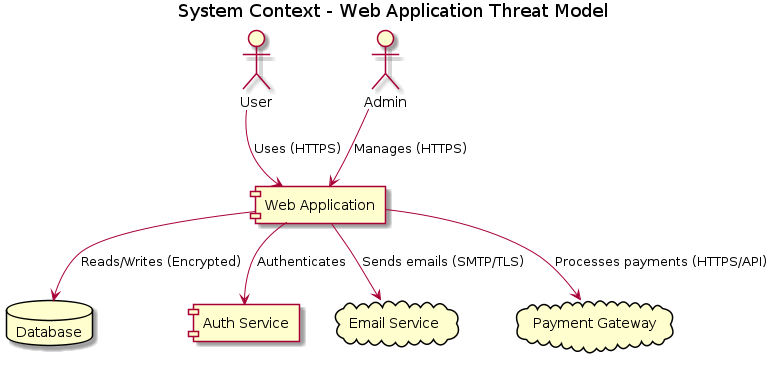
\includegraphics[width=0.8\textwidth]{images/system-context}
    \caption{System Context Diagram}
    \label{fig:system-context}
\end{figure}

\subsection{STRIDE Threat Analysis}
Using Microsoft's STRIDE methodology, we identified the following potential threats (Figure \ref{fig:stride-analysis}):

\begin{figure}[H]
    \centering
    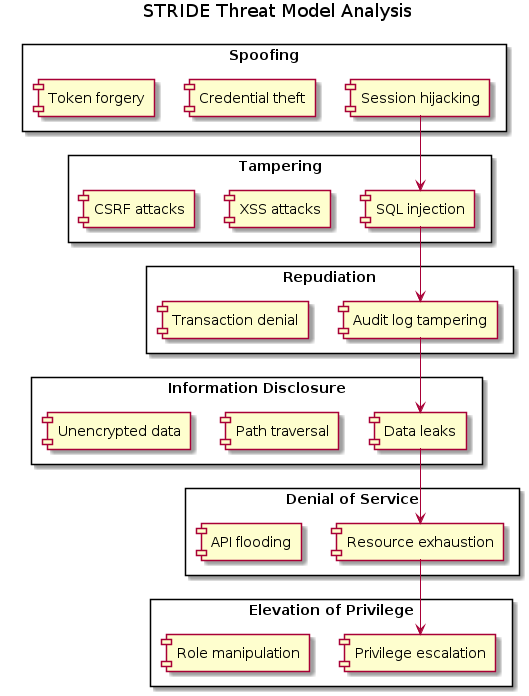
\includegraphics[width=0.8\textwidth]{images/stride-analysis}
    \caption{STRIDE Threat Analysis}
    \label{fig:stride-analysis}
\end{figure}

\section{Detailed Threat Analysis}

\subsection{Authentication and Authorization Threats}
\begin{itemize}
    \item \textbf{Threat:} Session hijacking through token theft
    \item \textbf{Impact:} Unauthorized access to user accounts
    \item \textbf{Controls:}
    \begin{itemize}
        \item Implement secure session management
        \item Use HTTP-only cookies
        \item Employ token rotation
    \end{itemize}
\end{itemize}

\subsection{Data Integrity Threats}
\begin{itemize}
    \item \textbf{Threat:} SQL injection attacks
    \item \textbf{Impact:} Unauthorized data access or modification
    \item \textbf{Controls:}
    \begin{itemize}
        \item Use parameterized queries
        \item Input validation
        \item Least privilege database access
    \end{itemize}
\end{itemize}

\subsection{Availability Threats}
\begin{itemize}
    \item \textbf{Threat:} DDoS attacks
    \item \textbf{Impact:} Service disruption
    \item \textbf{Controls:}
    \begin{itemize}
        \item Rate limiting
        \item DDoS protection services
        \item Load balancing
    \end{itemize}
\end{itemize}

\section{Security Controls and Mitigations}

\subsection{Implemented Controls}
\begin{enumerate}
    \item \textbf{Authentication}
    \begin{itemize}
        \item Multi-factor authentication
        \item Password complexity requirements
        \item Account lockout policies
    \end{itemize}
    
    \item \textbf{Authorization}
    \begin{itemize}
        \item Role-based access control
        \item Principle of least privilege
        \item Regular permission audits
    \end{itemize}
    
    \item \textbf{Data Protection}
    \begin{itemize}
        \item TLS 1.3 for data in transit
        \item AES-256 for data at rest
        \item Regular security audits
    \end{itemize}
\end{enumerate}

\section{Risk Assessment Matrix}

\begin{table}[H]
\centering
\begin{tabular}{|l|l|l|l|}
\hline
\textbf{Threat} & \textbf{Likelihood} & \textbf{Impact} & \textbf{Risk Level} \\
\hline
SQL Injection & High & Critical & High \\
Session Hijacking & Medium & High & High \\
DDoS Attack & High & Medium & Medium \\
Data Breach & Medium & Critical & High \\
\hline
\end{tabular}
\caption{Risk Assessment of Identified Threats}
\end{table}

\section{Implementation Plan}

\subsection{Phase 1: Critical Controls}
\begin{itemize}
    \item Implement WAF (Web Application Firewall)
    \item Deploy MFA for all administrative access
    \item Establish secure coding guidelines
\end{itemize}

\subsection{Phase 2: Enhanced Security}
\begin{itemize}
    \item Implement continuous security monitoring
    \item Deploy intrusion detection systems
    \item Regular penetration testing
\end{itemize}

\subsection{Phase 3: Maintenance}
\begin{itemize}
    \item Regular security assessments
    \item Update threat models
    \item Security awareness training
\end{itemize}


\section{Code Example: Vulnerable Login}

\begin{verbatim}
@app.route('/login', methods=['POST'])
def login():
    username = request.form['username']
    password = request.form['password']
    user = db.query(User).filter_by(username=username, password=password).first()
    if user:
        session['user_id'] = user.id
        return redirect('/dashboard')
    return 'Login failed', 401
\end{verbatim}

	extbf{Threats:} Susceptible to SQL injection, credential stuffing, and session fixation.\\
	extbf{Mitigations:} Use parameterized queries, hash passwords, implement account lockout, and use secure session cookies.

\section{Lab/Simulation}
To simulate a threat model:
\begin{enumerate}
    \item Clone this repo and install PlantUML and LaTeX.
    \item Generate diagrams:
    \begin{verbatim}
    plantuml system-context.puml
    plantuml stride-analysis.puml
    mv *.png images/
    \end{verbatim}
    \item Compile the report:
    \begin{verbatim}
    pdflatex threat-model.tex
    bibtex threat-model
    pdflatex threat-model.tex
    pdflatex threat-model.tex
    \end{verbatim}
\end{enumerate}

\bibliographystyle{alpha}
\bibliography{sample}

\end{document}
